\documentclass[10pt,a4paper]{article}
\usepackage[utf8]{inputenc}
\usepackage[french]{babel}
\usepackage[T1]{fontenc}
\usepackage{amsmath}
\usepackage{amsfonts}
\usepackage{amssymb}
\usepackage{graphicx}
\usepackage{physics}
\usepackage[lofdepth,lotdepth]{subfig}
\usepackage[left=2cm,right=2cm,top=2cm,bottom=2cm]{geometry}
\author{Loann Brahimi}
\title{Détermination du taux de turbulence des ondes de Alfvén par équilibre du taux de croissance et d'amortissement des ondes de Alfvén dans les milieux faiblement ionisés}
\begin{document}
\maketitle

\section{Modes de Alfvén et niveau de turbulence}

Dans cette partie nous ajoutons l'effet de la viscosité des neutres. Pour cela nous devons conserver l'expression la plus générale de la relation de dispersion des ondes de Alfvén c'est à dire incluant les collisions ion-neutres ainsi que la viscosité des neutres (Xu+2015b) : 

\begin{equation}
	\omega^3 + i (\tau_v^{-1} + (1 + \chi)\nu_{ni}) \omega^2 - (k^2\cos^2\theta V_{Ai}^2 + \chi \tau_v^{-1} \nu_{ni})\omega - i(\tau_v^{-1} + \nu_{ni}) k^2 \cos^2\theta V_{Ai}^2 = 0
\end{equation}

où $\tau_v^{-1} = k^2 \nu_n$ est la fréquence de collision des neutres, et $\nu_n = c_n^2 / (\nu_{nn} n_n)$. Les différents paramètres sont donnés dans notre cas particulier d'un milieu faiblement ionisé par : $c_n = 9.79\times 10^5 (\mathrm{cm}~\mathrm{s}^{-1}) \sqrt{\gamma_{ad}/\mu_n} (T / 1~\mathrm{eV})^{1/2}$, $\gamma_{ad} = 5/3$, $\mu_n = m_n / m_H$ et enfin $\nu_{nn} = 1.5 \times 10^{-10} (T/ 1~\mathrm{K})^{0.31} ~ \mathrm{cm}^3\mathrm{s}^{-1}$. \\ 

Dans le cas où l'on considère un faible amortissement des ondes de Alfvén ie. $\abs{\Gamma} \ll \abs{\omega_R}$, les solutions analytiques ($\omega = \omega_R + i \Gamma$) de la relation de dispersion sont : 


\begin{eqnarray}
	\omega_R^2 & = & \frac{(k^2\cos^2\theta V_{Ai}^2 + \chi \tau_v^{-1} \nu_{ni})^2 + (\tau_v^{-1} + (1+\chi) \nu_{ni})(\tau_v^{-1}+\nu_{ni}) k^2 \cos^2\theta V_{Ai}^2}{\chi \tau_v^{-1} \nu_{ni} + k^2 \cos^2 \theta V_{Ai}^2 + (\tau_v^{-1} + (1 + \chi) \nu_{ni})^2} \\	
	\Gamma     & = & -\frac{[\tau_v^{-1}(\tau_v^{-1} + (1 + \chi)\nu_{ni}) + k^2 \cos^2 \theta V_{Ai}^2 ] \chi \nu_{ni}}{2 [k^2 \cos^2 \theta V_{Ai}^2 + \chi \tau_v^{-1} \nu_{ni} + (\tau_v^{-1} + (1+\chi)\nu_{ni})^2]} 
\end{eqnarray}

Les taux respectifs aux couplages faible et fort des ions avec les neutres sont présentés dans le tableau suivant : 
 
\begin{center}
\begin{tabular}{|c|c|c|c|}
\hline 
 & & Couplage i-n fort & Couplage i-n faible \\ 
 
& & $\omega \ll \nu_{in}$ & $\omega \gg \nu_{in}$ \\ 
\hline 
$\nu_n \neq 0$ &$\omega_R^2$ & $\xi_n^2k^4\nu_n^2 + k^2\cos^2\theta V_{A}^2$ & $k^2\cos^2\theta V_{Ai}^2$ \\ 

&$\Gamma$ & $- \frac{\xi_n}{2}\left( \frac{k^2 \nu_n}{\chi} + \frac{k^2 \cos^2\theta V_{A}^2 }{\nu_{ni}} \right)$ & $-\frac{\nu_{in}}{2}$ \\ 
\hline
$\nu_n = 0$ &$\omega_R^2$ & $k^2\cos^2\theta V_{A}^2$ & $k^2\cos^2\theta V_{Ai}^2$ \\

&$\Gamma$ & $-\frac{\xi_n k^2 \cos^2\theta V_{A}^2 }{2\nu_{ni}}$ & $-\frac{\nu_{in}}{2}$ \\

\hline 
\end{tabular}
\end{center} 

Dans le cas où l'on considère que la viscosité des neutres est nulle, il existe théoriquement une région de fort amortissement ie. $\abs{\Gamma} = \omega_R$  donnée par les nombres d'onde : $k_c^+ = \frac{2\nu_{ni}}{V_A\xi_n \cos\theta}$ et $k_c^- = \frac{\nu_{in}}{2V_{Ai}\cos\theta}$ (Xu+2015a). 

\section{Validité des différents régimes d'approximation} 
Dans cette section, nous allons à partir de l'analyse proposée par Xu+2015 discuter des différents régimes de couplage des ions avec les neutres et de la validité de l'approximation $\abs{\Gamma} \ll \omega_R$. Pour cela, nous prenons en exemple la relation de dispersion obtenue pour la phase WNM (figure \ref{fig:disp_WNM}). Nous n'avons considéré que l'amortissement par collisions ions-neutres. En haut à gauche nous avons les valeurs exactes de $\omega_R$ et $\Gamma$ telles qu'elles sont présentées dans la première section. On observe globalement que $\abs{\Gamma} \ll \omega_R$ ce qui signifie que l'approximation de faible amortissement est justifiée. \\ 

En ce qui concerne le domaine du couplage faible (en bas à gauche), on voit que $\abs{\Gamma} \ll \omega_R$ jusqu'à une certaine valeur qui ne correspond à aucune des deux valeurs de l'intervalle de coupure, il faut donc déterminer de manière plus précise à valeur à partir de laquelle l'amortissement des modes de Alfvén devient de l'ordre de la pulsation des ondes. On voit clairement qu'à haute énergie, l'approximation de faible amortissement n'est plus valable en faible couplage. \\ 

Le cas du couplage fort (en haut à droite) est problématique. On observe que $\abs{\Gamma} \gg \omega_R$ sur tout l'intervalle d'étude. On pourrait en déduire que l'approximation de couplage fort ($\nu_{ni} \gg \omega$) n'est pas valable. Cependant on observe clairement que $\nu_{ni} \sim 10^{-11} ~ \mathrm{s}^{-1}$ alors que $\omega_R \sim 10^{-27} - 10^{-12}~\mathrm{s}^{-1}$. Une autre possibilité est que l'approximation $\abs{\Gamma} \ll \omega_R$ n'est pas valable en couplage fort, il est donc intéressant d'étudier la relation de dispersion (19) de Xu+2015b de la manière la plus générale possible. 

\begin{center}
	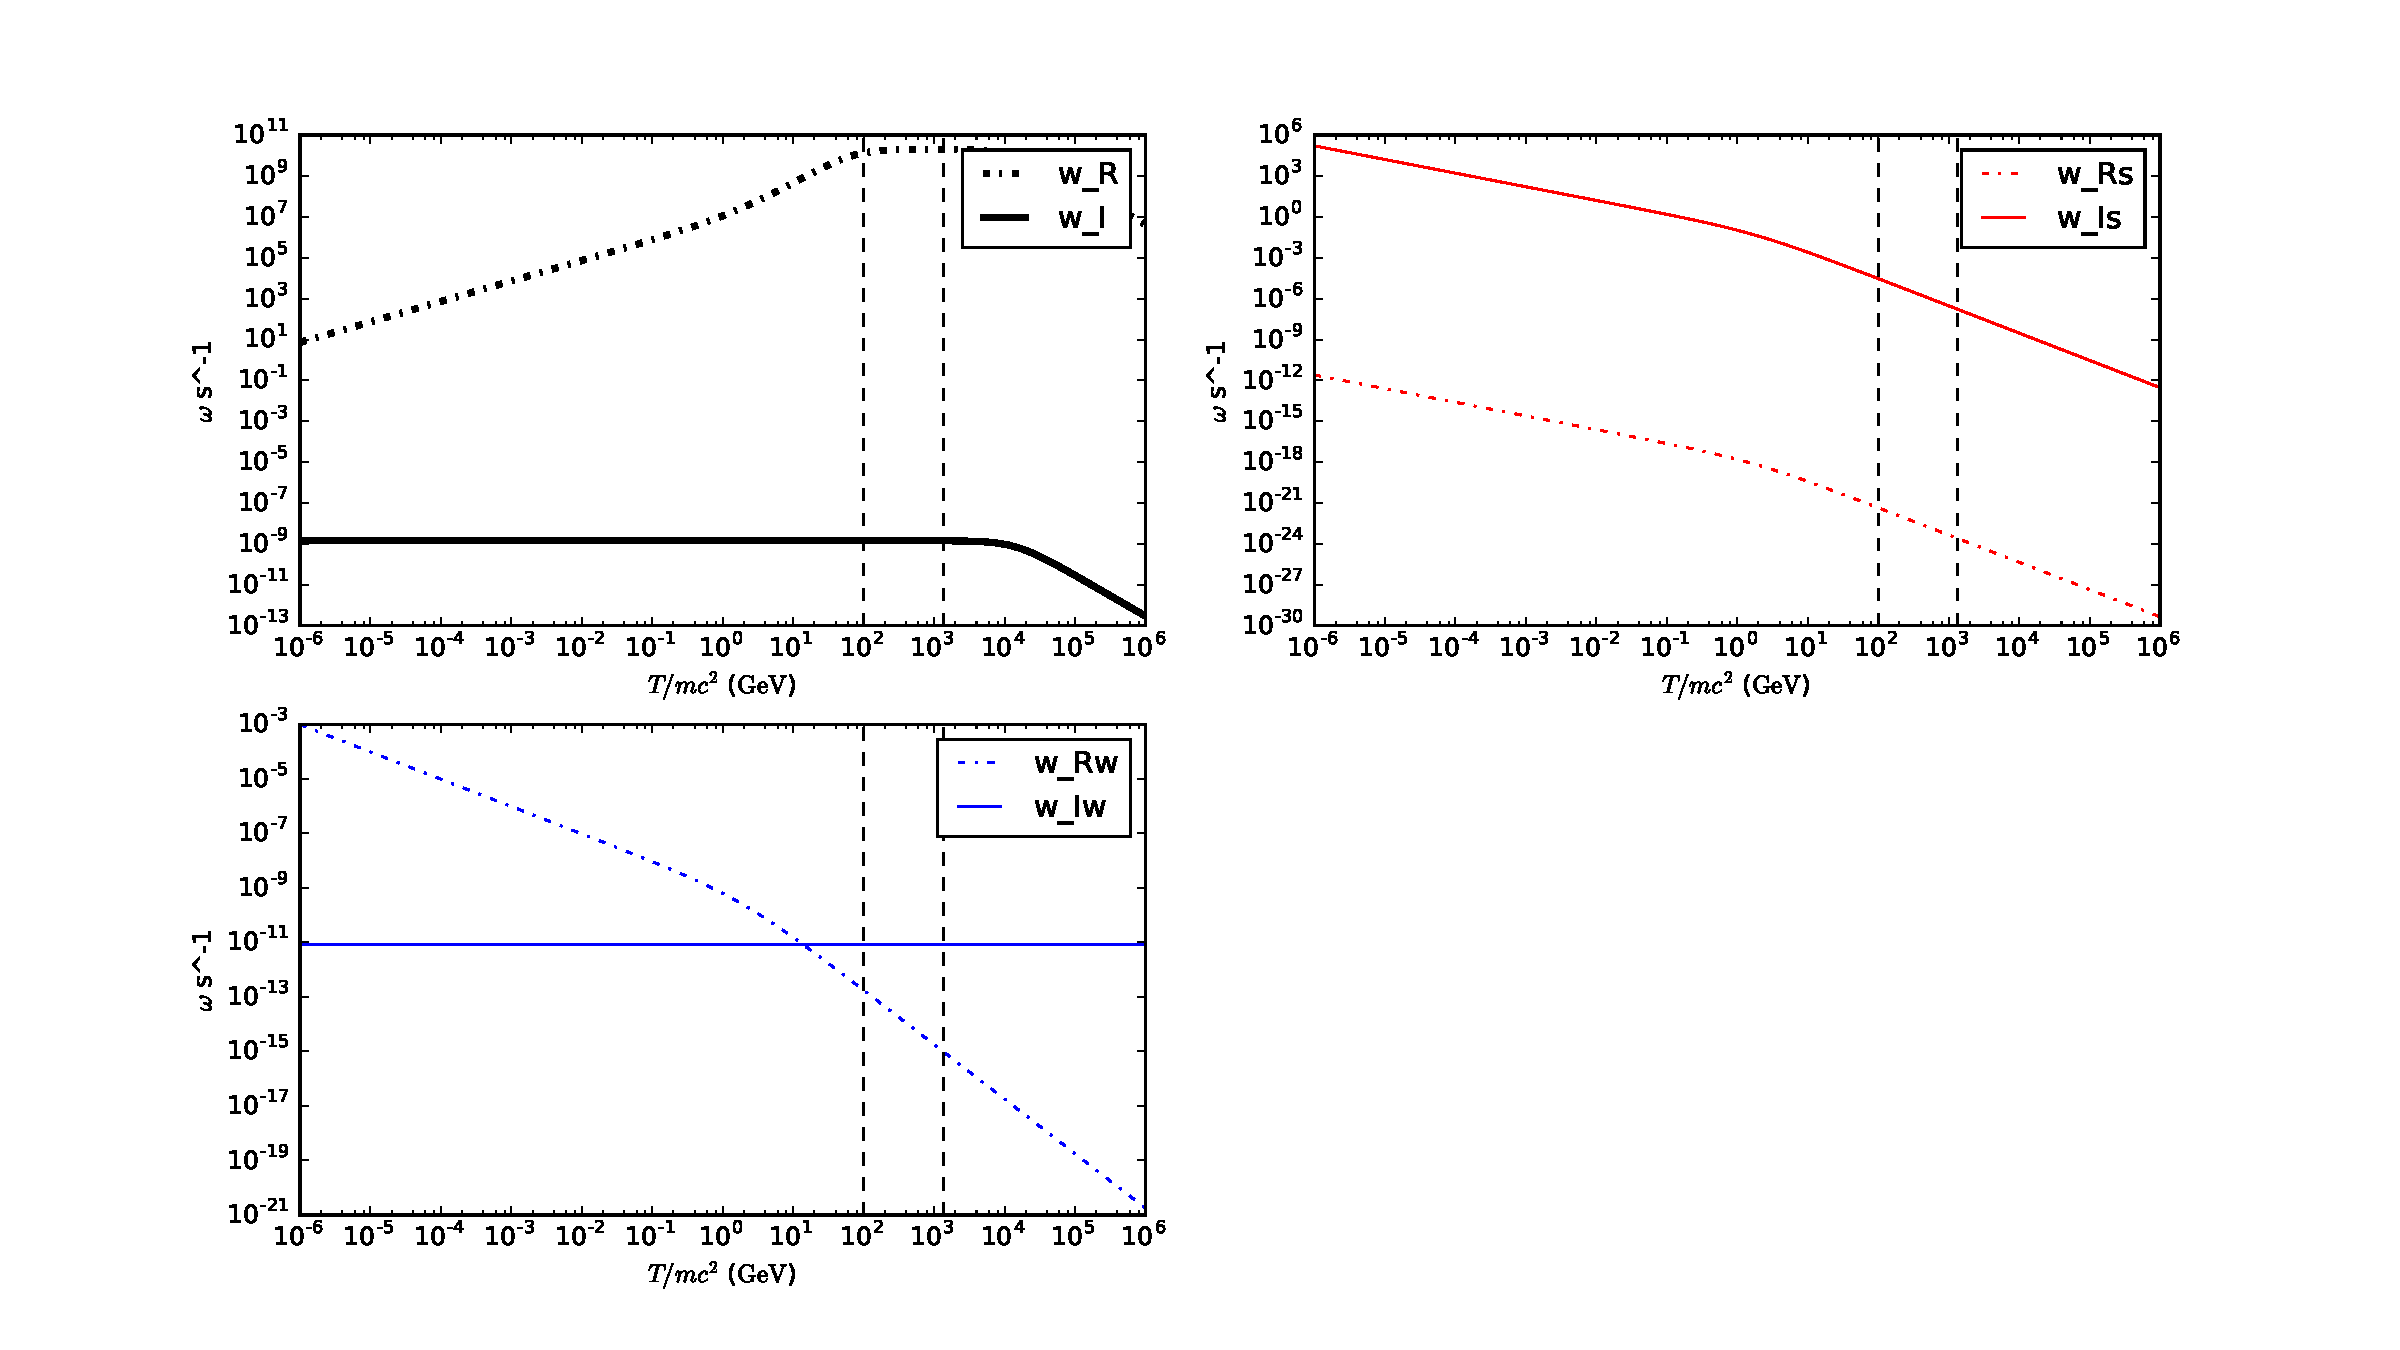
\includegraphics[scale=0.4]{./figures/WNM_dispersion.pdf}
	\label{fig:disp_WNM}
\end{center}


\end{document}